%!TEX root = /Users/domaubert/Documents/Lectures/cosmologie/cosmo_main.tex

\chapter{Formation des grandes structures}
\label{s:struct}
\begin{figure}[htbp]
	\centering
		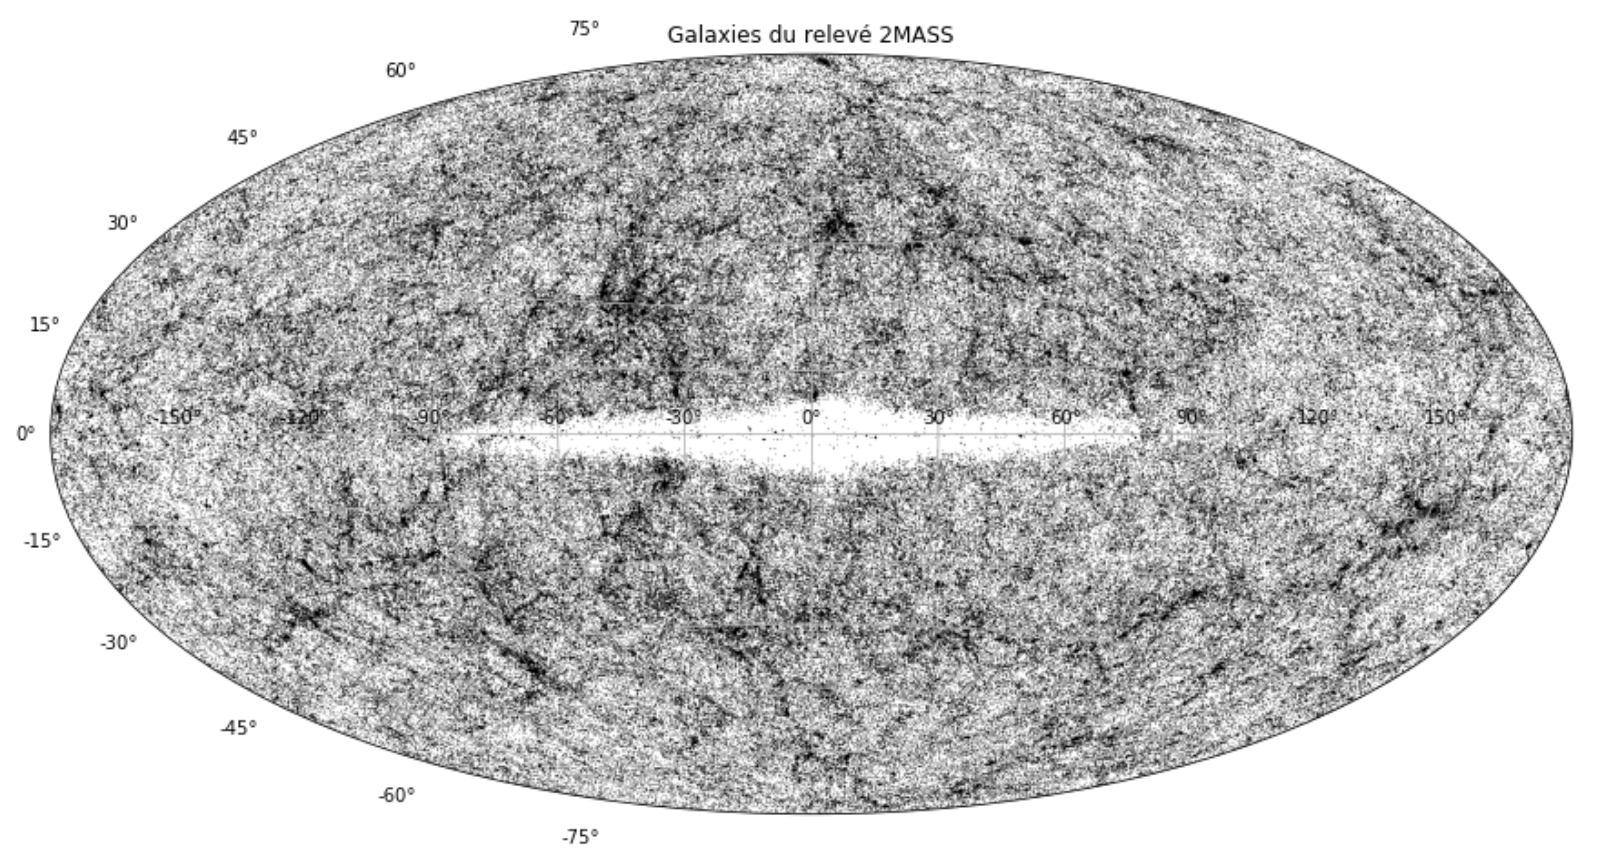
\includegraphics[height=12cm]{figs/2MASSLSS.png}
		\caption[Le relevé de galaxies 2MASS]{La distribution sur le ciel de 550 000 galaxies du grand relevé infrarouge 2MASS, telle qu'elle serait vue par un observateur au centre de la Voie Lactée. Chaque point est une galaxie distante : ces galaxies sont distribuées le long des \textit{grandes structures de l'Univers} qui combinent régions denses, grands vides et filaments de matière. On note un déficit d'objets au centre de l'image, due à la présence de la Voie Lactée qui bloque les lignes de visée.}
	\label{f:2MASS}
\end{figure}

Les grandes structures de l'Univers\index{grandes structures de l'Univers} désignent de façon générique et tout à la fois la matière diffuse, les galaxies et amas de galaxies qui s'organisent sous l'effet de la gravitation. Aujourd'hui, ces grandes structures produisent une distribution de matière 'filamentaire' où des surdensités côtoient des vides, reliées entre elles par des ponts de matériau. Elles résultent de l'action du mécanisme d'instabilité gravitationnelle\index{instabilité gravitationnelle} sur les faibles fluctuations de densité présentes dans l'Univers jeune et tracées par exemple par le CMB. Au cours des 13.8 milliards d'années, des surdensités de 0.001\% parviennent ainsi à croître pour atteindre des contrastes de densité mesurés d'au moins plusieurs centaines dans les galaxies aujourd'hui. Si une grande partie des processus à l'œuvre lors de la formation des grandes structures peuvent être saisis par une approche analytique, le problème ne peut être abordé dans toute sa complexité que via l'utilisation de simulations numériques, dites simulations cosmologiques\index{simulation cosmologique}.


\begin{figure}[htbp]
	\centering
		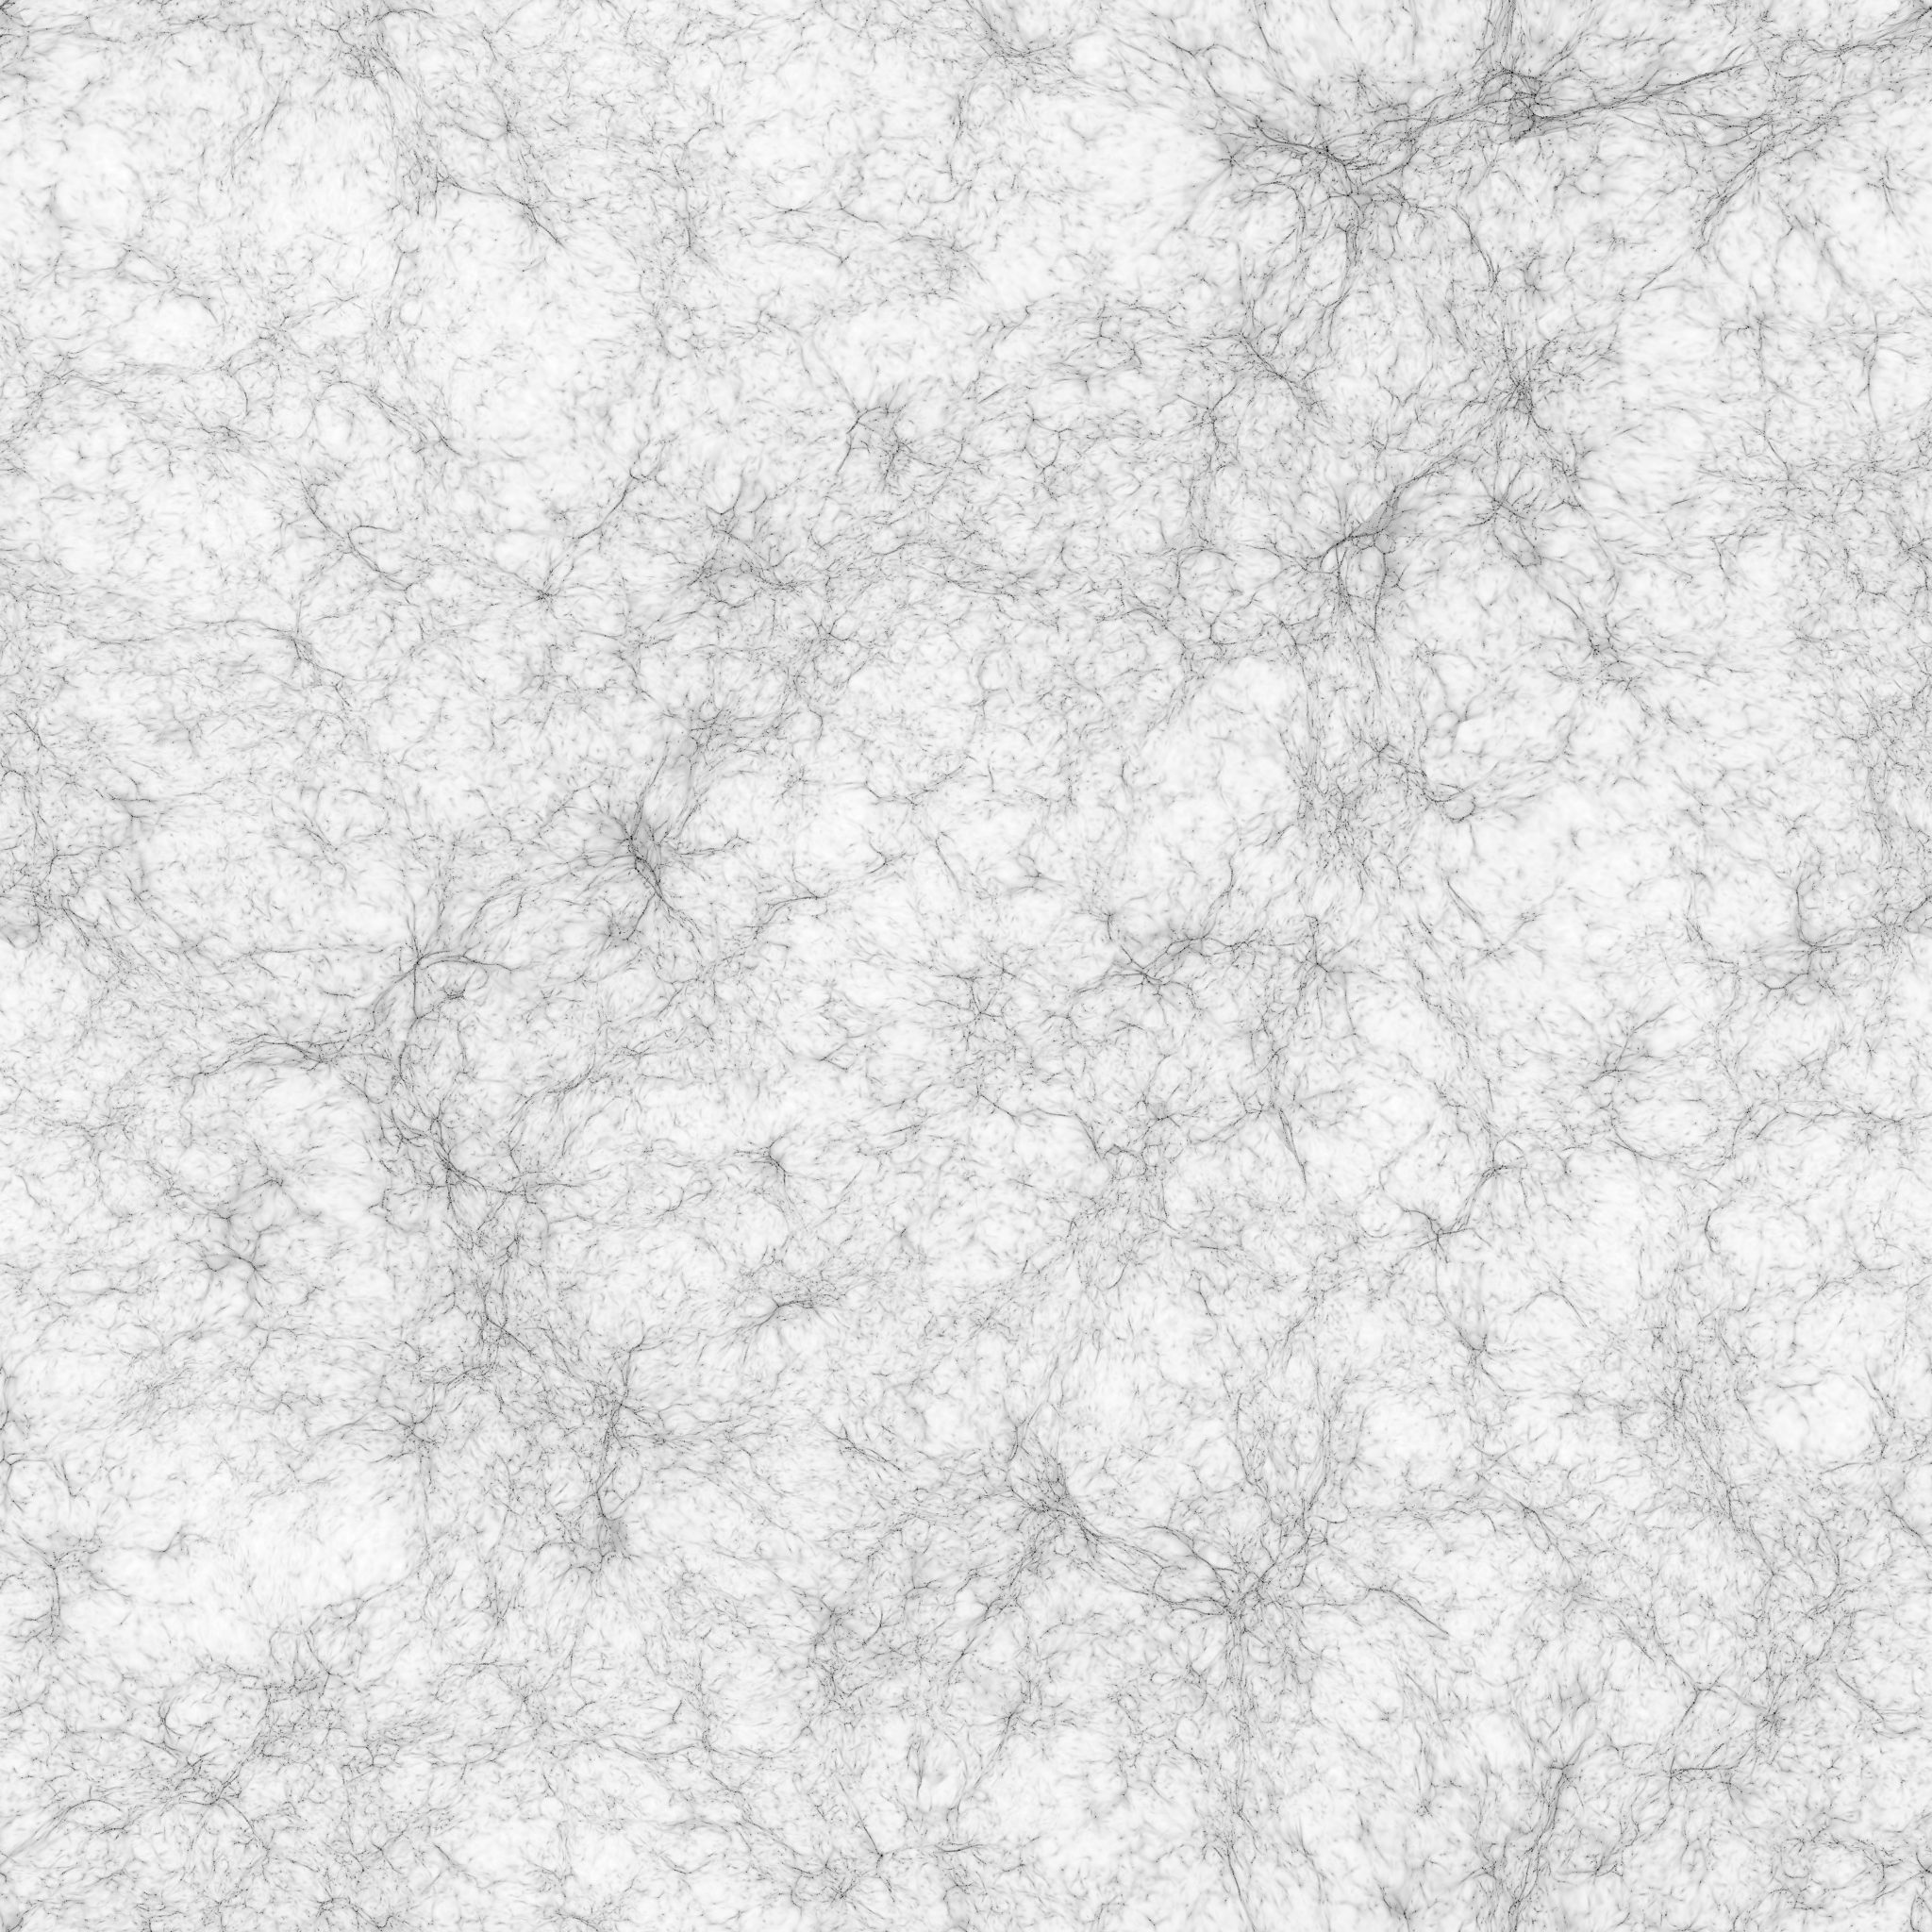
\includegraphics[height=12cm]{figs/simLSS.png}
		\caption[Simulation des grandes structures de l'Univers]{La distribution de la matière telle qu'elle est prédite par une simulation cosmologique de formation des grandes structures. Ce carré fait environ 100 Mpc de côté et correspond à un Univers jeune, 1 milliard d'années après le Big-Bang ($z\sim 6$). On retrouve la distribution typique en vides, amas et filaments qui est observée dans le ciel}
	\label{f:simLSS}
\end{figure}


\section{Densité et spectre de puissance}
L'un des objectifs de l'étude de la formation des grandes structures est de prédire comme la matière va s'organiser au cours de l'histoire de l'Univers. La quantité généralement suivie est le contraste de densité\index{contraste de densité} :
\begin{equation}
\delta(x,t) =\frac{\rho-\bar\rho}{\bar\rho}.
\end{equation}
En l'absence de création de masse et dans un Univers homogène et isotrope, la densité moyenne $\bar{\rho}$ est une quantité de référence constante dans l'espace et pour laquelle la variation temporelle est seulement due à la dilution cosmologique \sidenote{dont on rappelle qu'elle fait varier la densité en $a^{-3}$.}

Toutefois, le contraste de densité à une position $x$ donnée et à un instant donné $t$ est finalement porteur d'assez peu d'information cosmologique, puisque l'on cherche à obtenir des contraintes qui ont des valeurs globales et génériques. La première étape vers un traitement cosmologique consiste à raisonner dans l'espace de Fourier\index{transformée de Fourier} et à considérer les \textit{modes} $\delta_k(t)$ d'une réalisation donnée de $\delta(x,t)$:
\begin{equation}
\delta(x,t)\sim\int_{k=-\infty}^\infty \delta_k(t) e^{ikx} dk.
\label{e:fourdelta}
\end{equation}
L'équation \ref{e:fourdelta} représente la décomposition en série de Fourier du contraste de densité : en pratique cela revient à décomposer le champ de densité en une série de modes sinusoïdaux et dont les contributions des différentes fréquences sont données par $\delta_k$. En plus d'un intérêt mathématique, cette décomposition constitue une mise en pratique de 'cosmologisation' de la densité : on se met à suivre des modes sinusoïdaux délocalisés, de taille caractéristique $\lambda=2\pi/k$\sidenote{$\lambda$ qui est donc la longueur d'onde} et la position $x$ perd de l'importance en tant que telle. L'amplitude d'un mode $k$ est donnée tout simplement par $|\delta_k|^2$: l'étude de cette amplitude et son éventuelle évolution temporelle nous renseigne globalement sur l'évolution des structures d'échelle caractéristique $\lambda$ au cours du temps et sur leurs contributions relatives. Cette amplitude est aussi appelée \textit{puissance} et l'ensemble des puissances de tous les modes $k$ est appelé \textit{spectre de puissance}\index{spectre de puissance}.

\paragraph{Champ aléatoire Gaussien} Le champ de matière cosmologique appartient semble-t-il à la classe des champs aléatoires gaussiens\index{champs aléatoire gaussien}. C'est une prédiction des théories inflationnaires et il semble observationnellement que ce soit le cas : in fine, cela constitue une base de travail et éventuellement on pourra être amené à mesure des départs à cette gaussianité. Un champ aléatoire gaussien $\delta(\vec x)$ se caractérise par une densité de probabilité (PDF) \index{densité de probabilité} de type:
\begin{equation}
p(\delta(\vec x)) \sim \exp( -\delta (\vec x) C^{-1} \delta (\vec x)),
\end{equation}
où $C$ est une matrice de corrélation, généralement non diagonale. Cette matrice encode les corrélations qui peuvent apparaître dans le champ de matière : celui-ci possède généralement des structures possédant une certaine cohérence spatiale et cette dernière se manifeste en couplant le champ $\delta$ entre différentes positions via $C$ \sidenote{par exemple la structuration de la matière dans l'Univers est telle que les régions denses se trouvent plutôt à proximité d'autres régions denses.}. Une propriété intéressante est que la densité de probabilité de la transformée de Fourier de $\delta (\vec x)$ suit le même type de PDF:
\begin{equation}
p'(\delta_{\vec k})\sim \exp( -\delta_{\vec k}^* \tilde C^{-1} \delta_{\vec k}).
\end{equation}
Une propriété encore plus intéressante est que $\tilde C$ est diagonale si $\delta(\vec x)$ est un champ aléatoire gaussien: chaque mode de Fourier peut être suivi statistiquement indépendamment des autres. Par simple inspection, il apparaît que les composantes de cette matrice de corrélation sont les variances des modes\sidenote{ici $\delta_D$ désigne la fonction de Dirac, nulle partout sauf en 0, telle que $\int_{-\infty}^{\infty} dx \delta_D(x)=1$}:
\begin{equation}
\langle \delta_{\vec k}^* \delta_{\vec k'}\rangle = P(k)\delta_D(\vec k -\vec k')=\langle|\delta_{\vec k}|^2\rangle.
\end{equation}
Cette mesure de la variance ne dépend que la norme $k=|\vec k|$ du mode considéré (plusieurs modes de directions différentes, mais de modules identiques partagent donc la même variance du fait de l'isotropie) et constitue le spectre de puissance $P(k)$\index{spectre de puissance} du champ de matière.

Cette quantité est destinée à être mesurée au cours du temps et nous renseigne sur la croissance des structures. Si certaines échelles bénéficient d'une croissance plus rapide que d'autres, cela se manifestera par une déformation du spectre de puissance aux échelles concernées.  Si le champ est vraiment un champ aléatoire gaussien, la connaissance de sa variance et donc de $P(k)$ suffit à complètement le définir : si des corrélations anisotropes sont détectées (dans les relevés de galaxies ou dans le CMB), elles confirmeront soit la nature non gaussienne\index{non-gaussianité} des fluctuations primordiales soit l'existence de processus physiques qui génèrent de la non-gaussianité \sidenote{notons que le spectre de puissance ne permet pas de mesurer la non-gaussianité. Deux champs, l'un gaussien l'autre non, peuvent partager les mêmes variances. Il faut utiliser des statistiques d'ordres supérieurs pour pouvoir faire cette distinction.}.

Une quantité reliée au spectre de puissance est la fonction de corrélation à deux points\index{fonction de corrélation} $\xi (r)$: elle exprime l'excès de probabilité de trouver de la matière en deux points séparés d'une certaine distance $r$ par rapport à une distribution aléatoire. On peut démontrer que la fonction de corrélation à deux points est simplement la représentation du spectre de puissance dans l'espace des positions (donc sa transformée de Fourier):
\begin{equation}
\xi (r)\sim \int d\vec k P(k) e^{i k r}.
\end{equation}
Notons qu'à nouveau cet excès de probabilité ne dépend que de la distance $r$ et non pas d'une orientation ou de positions spécifiques des 2 points considérés. Généralement, la fonction de corrélation à 2 points est utilisée si l'on a une description discrète du champ de densité: c'est le cas par exemple lorsque l'on utilise des galaxies comme traceurs de la matière dans les grands relevés. Si l'on travaille avec un champ continu (comme dans des travaux analytiques), on passe directement dans une représentation en mode de Fourier en utilisant le spectre de puissance $P(k)$: ce dernier présente l'avantage d'explicitement séparer les modes de tailles différentes, là où la fonction de corrélation à 2 points "mélange" les modes et peut donc être dominée par une échelle au détriment des autres, qui peuvent pourtant contenir une information pertinente.

\section{Longueur de Jeans}
Une quantité centrale dans l'étude de l'instabilité gravitationnelle est la longueur de Jeans\index{longueur de Jeans}\sidenote{voir aussi le chapitre dédié à la matière noire}, notée $\lambda_J$. Elle correspond à la longueur minimale  que doit avoir une structure pour s'effondrer sous l'effet de la gravitation. On y associe également une masse (la masse de Jeans\index{masse de Jeans}) $M_J$ donnée simplement par:
\begin{equation}
M_J=\frac{4\pi}{3}\bar\rho\lambda_J^3,
\end{equation}
,où $\bar \rho$ est la densité moyenne du milieu : une structure de masse supérieure à la masse de Jeans va s'effondrer. L'existence d'une grandeur critique pour que l'effondrement se réalise traduit l'existence d'une compétition entre la gravité et un autre processus que la gravité doit 'vaincre'. En général, cet autre processus est l'existence d'un support thermique qui fournit une pression à même de s'opposer à la gravitation. Pour du gaz, il s'agit généralement de la pression interne du gaz, pour des systèmes non-collisionnels (type gaz d'étoiles) c'est la dispersion de vitesse interne qui agit comme une barrière à l'effondrement\sidenote[][-2cm]{voir aussi le chapitre dédié à la matière noire}.

L'expression de la longueur de Jeans peut s'obtenir avec un simple raisonnement: pour qu'une structure s'effondre il faut que l'information gravitationnelle se répartisse plus rapidement au sein d'une structure que l'information de support thermique. Dans un milieu de densité $\rho$ l'information gravitationnelle est transportée en un temps dynamique\index{temps!dynamique}
\begin{equation}
t_G\approx \frac{1}{\sqrt{G\rho}}.
\end{equation}
Pour un gaz, la transmission de l'information de support thermique dépend de la vitesse du son\index{vitesse!du son} $c_s$ et de la taille de la structure $\lambda$:
\begin{equation}
t_p\approx\frac{\lambda}{c_s}.
\end{equation}
L'effondrement a lieu si $t_G<t_p$, donc si la taille de la structure considérée obéit à la condition:
\begin{equation}
\lambda >\frac{c_s}{\sqrt{G\rho}}\equiv \lambda_J.
\end{equation}
Faire baisser $\lambda_J$ revient à favoriser l'effondrement gravitationnel, le cas limite étant $\lambda_J \rightarrow 0$ où toute structure s'effondre. Ce régime s'obtient dans un milieu très dense ou bien très froid, c.-à-d. sans support thermique.  À l'inverse, une grande valeur de $\lambda_J$ réduit la possibilité d'effondrement et $\lambda_J\rightarrow\infty$ revient à empêcher toute structure de s'effondrer: cela correspond à un milieu sous-dense, donc très léger, ou bien très chaud avec une grande vitesse du son. Pour un système non collisionnel, la même expression existe pour la longueur de Jeans en remplaçant la vitesse du son par la dispersion de vitesse du milieu.

%\subsection{Traitement perturbatif}
Une dérivation plus rigoureuse peut être obtenue par un traitement perturbatif au premier ordre. On considère un gaz de densité moyenne $\bar \rho$ et d'équation d'état reliant\sidenote{ici $P$ désigne la pression du gaz. Notons par exemple que dans le cas du gaz parfait $P=\rho k_B T$, nous avons $k_B T\sim c_s^2$ qui est conforme à cette formulation d'une équation d'état}:
\begin{equation}
\frac{dP}{d\rho}=c_s^2.
\end{equation}
Ce gaz obéit à l’équation de Poisson\index{equation@équation!de Poisson}, qui est l'équation de champ de la gravité newtonienne liant potentiel $\phi$ et densité:
\begin{equation}
\Delta \phi(x,t) = 4 \pi G \rho
\end{equation}
 et aux équations fluides, conservation de la masse\index{conservation de la masse}\sidenote{ici $u$ désigne la vitesse du fluide}
 \begin{equation}
 \frac{\partial \rho}{\partial t} + \vec \nabla \rho \vec u=0,
 \end{equation}
 et conservation de l'impulsion\index{conservation de l'impulsion}
 \begin{equation}
 \frac{\partial \vec v}{\partial t} +\vec u \vec \nabla \vec u = -\frac{\vec \nabla P}{\rho}-\vec \nabla \phi.
 \end{equation}
 On réalise un traitement perturbatif (à 1D par simplicité)\sidenote{notons qu'on considère ici que le milieu n'est pas animé d'une vitesse globale à l'équilibre $v_0=0$ et que le milieu à l'équilibre ne présente pas de variations spatiales de potentiel : ce potentiel $\phi_0$ constant dans l'espace est sans influence dynamique et est donc ignoré. Les quantités $\delta,v_1,\phi_1, P_1$ sont des petites quantités}:
 \begin{eqnarray}
 \rho(x,t)&=&\bar \rho(1 +\delta(x,t))\\
 u(x,t)&=&v_1(x,t)\\
 \phi(x,t)&=&\phi_1(x,t)\\
 P&=&P_0+P_1(x,t)
 \end{eqnarray}
 En injectant ces développements, on parvient aisément à écrire:
 \begin{eqnarray}
 \frac{\partial \delta}{\partial t}&=&-\bar \rho \frac{\partial v_1}{\partial x}\\
 \frac{\partial}{\partial t}\frac{\partial v_1}{\partial x}+\frac{c_s^2}{\bar \rho}\frac{\partial^2 \delta}{\partial x^2}+\frac{\partial^2 \phi_1}{\partial x^2}&=&0
 \end{eqnarray}
 d'où l'équation maîtresse de l'instabilité:
 \begin{equation}
 \ddot \delta -c_s ^2\frac{\partial^2 \delta}{\partial x^2}=4\pi G \bar \rho \delta
 \end{equation}
 \subsection{Effondrement et Oscillations}
 Cette équation s'analyse plus facilement en prenant sa transformée de Fourier\index{transformée de Fourier} spatiale:
 \begin{equation}
 \ddot \delta_k +(c_s^2k ^2-4\pi G \bar \rho) \delta_k= 0.
 \end{equation}
 Deux régimes peuvent être facilement distingués:
 \begin{itemize}
 \item si $c_s^2 k^2> 4\pi G \bar \rho$ c'est une équation d'oscillateur harmonique\index{oscillateur harmonique}. Le mode correspond à une onde sonore en $e^{i\omega t}$ de pulsation\sidenote{et donc de fréquence temporelle $\nu=2\pi/\omega$} $\omega=\sqrt{c_s^2 k^2-4\pi G \bar \rho}$. Cela correspond à des grandes fréquences spatiales, donc des petites structures: notons que la pulsation est d'autant plus grande que ces structures sont petites.
 \item si $c_s^2 k^2< 4\pi G \bar \rho$, la solution est hyperbolique avec une contribution exponentielle croissante en $e^{t/\tau}$, qui correspond à l'instabilité gravitationnelle\index{instabilité gravitationnelle}. Ce régime correspond aux faibles valeurs de $k$ donc aux grandes échelles. Le temps caractéristique d'instabilité est $\tau = (4\pi G \bar \rho - c_s^2k^2)^{-1/2}$ qui se résume au temps dynamique\index{temps dynamique}\sidenote{c'est à dire $1/\sqrt{G\rho}$} si k est suffisamment faible donc si le mode étudié est suffisamment grand. 
 \end{itemize}
 
 On remarque que le cas critique $\frac{4\pi^2c_s^2}{\lambda^2}=4\pi G \rho$ nous redonne la longueur de Jeans\index{longueur de Jeans}
 \begin{equation}
 \lambda_J=c_s\sqrt{\frac{\pi}{G\rho}}
 \end{equation}
 
 \subsection{Cas cosmologique}
\newthought{Le cas cosmologique} se doit de prendre en compte l'expansion de l'Univers. Comme on le verra en fin de démonstration, cela change finalement peu de choses par rapport au cas exposé précédemment. Toutefois, cette étude présente un intérêt technique en rapport avec la manipulation de grandeur comobiles dans des équations différentielles couplées. Pour cette raison, le calcul sera décrit en détail.

\newthought{Les équations importantes} sont les mêmes que dans le cas d'un Univers statique\sidenote{$\rho$ est la densité de matière, $\vec u$ la vitesse, $\vec  r$ la position physique, $P$ la pression et $\phi$ le potentiel gravitationnel}:
\begin{eqnarray}
\frac{\partial \rho}{\partial t}+\frac{\partial \rho \vec u}{\partial \vec r}&=&0\\
\frac{\partial \vec u}{\partial t}+\vec u \cdot \frac{\partial \vec u}{\partial \vec r}&=&-\frac{1}{\rho}\frac{\partial P}{\partial \vec r}-\frac{\partial \phi}{\partial \vec r}\\
\frac{\partial^2 \phi}{\partial \vec r^2}&=&4\pi G \rho.
\end{eqnarray}
 La principale difficulté découle de la dépendance temporelle de la distance physique\index{distance!physique} $\vec r=a(t) \vec x(t)$ où $\vec x$ désigne la position comobile\index{distance!comobile} : la dérivée par rapport à $\vec r$ doit donc être prise avec précaution. Par commodité on préfère généralement écrire ces équations en fonction de données comobiles pour extraire au moins l'effet de flot cosmologique encodé par le facteur d'expansion $a(t)$.
 
La première étape consiste à transformer les dérivées temporelles prises à $\vec r$ constant en dérivées prises à $\vec x$ constant\sidenote{on rappelle que pour $f(r=a(t)x,t)$ alors $\left(\frac{\partial f}{\partial t}\right)_x=\left(\frac{\partial f}{\partial t}\right)_r+\frac{\partial f}{\partial \vec r}\frac{\partial \vec r}{\partial t}$}:
\begin{equation}
\left(\frac{\partial }{\partial t}\right)_r = \left(\frac{\partial }{\partial t}\right)_x-\frac{\dot a}{a}\vec x \cdot \left(\frac{\partial}{\partial \vec x}\right)_t,
\end{equation}
de même, les dérivées spatiales deviennent:
\begin{equation}
\frac{\partial }{\partial \vec r}=\frac{1}{a}\frac{\partial}{\partial \vec x}.
\end{equation}
 Pour finir, il faut établir que la vitesse comporte une partie liée au flot de Hubble\index{Hubble!flot} \sidenote{ le terme $\dot a \vec x$ peut facilement se réécrire sous la forme $H \vec r$, c.-à-d. la loi de Hubble\index{loi de Hubble}}:
\begin{equation}
\dot {\vec u}=\dot a \vec x + a \dot {\vec x}= \dot a \vec x + \vec v
\end{equation}
 où $\vec v$ désigne une vitesse particulière superposée au flot cosmologique.
 Enfin, la densité sera également exprimée en fonction de la densité de fond, $\bar \rho \sim a^{-3}$ qui subit l'expansion cosmologique :
 \begin{equation}
 \rho(\vec x,t) =\bar \rho(t)(1+\delta(\vec x,t)).
 \end{equation}
 
 \newthought{La conservation de la masse}\index{conservation de la masse} est modifiée comme suit : nous allons prendre les différents termes un par un. La dérivée temporelle de la densité comprend 2 termes, le premier \sidenote{notez la dérivée temporelle de $\bar \rho\sim a^{-3}$ qui intervient ici }:
 \begin{eqnarray}
  \left(\frac{\partial \rho}{\partial t}\right)_x&=& \left(\frac{\partial \rho}{\partial t}\right)_r,\\
  &=&\bar \rho\frac{\partial \delta}{\partial t} -3\frac{\dot a}{a}\bar \rho (1+\delta),
 \end{eqnarray}
et le second:
\begin{eqnarray}
\frac{\dot a}{a}\vec x \cdot \frac{\partial \rho}{\partial \vec x}&=&\frac{\dot a }{a}\bar \rho \frac{\partial\delta}{\partial \vec x}.
\end{eqnarray}
Le terme de flux de cette même équation devient quant à lui:
\begin{eqnarray}
\frac{1}{a}\frac{\partial}{\partial \vec x}(\bar \rho(1+\delta)(\vec v + \dot a \vec x))&&\\
=\frac{\bar \rho}{a} \frac{\partial}{\partial \vec x}(\bar \rho(1+\delta)\vec v) + \frac{\bar \rho \dot a}{a} \frac{\partial}{\partial \vec x}(\bar \rho(1+\delta)\vec x)&&.
\end{eqnarray}
Le dernier terme de cette égalité peut être réécrit sous la forme:
\begin{eqnarray}
\frac{\bar \rho \dot a}{a} \frac{\partial}{\partial \vec x}(\bar \rho(1+\delta)\vec x)&&\\
=\bar \rho \frac{\dot a }{a} 3(1+\delta) +\bar \rho \frac{\dot a }{a} \vec x \cdot \frac{\partial \delta}{\partial \vec x}.
\end{eqnarray}
En rassemblant le tout on obtient l'équation de conservation de la masse dans sa formulation comobile:
\begin{equation}
\frac{\partial \delta}{\partial t}+\frac{1}{a}\frac{\partial}{\partial \vec x}((1+\delta)\vec v)=0
\end{equation}

 \newthought{L'équation d'Euler comobile}\sidenote{qui n'est autre qu'une équation de conservation de l'impulsion} \index{equation@équation!d'Euler} se dérive de la même manière. Prenons le premier terme de dérivée temporelle de la vitesse:
 \begin{eqnarray}
 \left(\frac{\partial \vec u}{\partial t}\right)_r&=&\left(\frac{\partial \vec u}{\partial t}\right)_x-\frac{\dot a }{a}\vec x \cdot \frac{\partial \vec u}{\partial \vec x}.
\end{eqnarray}  
La dérivée temporelle à $\vec x$ constant donne:
\begin{eqnarray}
\left(\frac{\partial \vec u}{\partial t}\right)_x&=&\left(\frac{\partial \vec v}{\partial t}\right)_x + \ddot a {\vec x},
\end{eqnarray}
tandis que le terme de Hubble donne \sidenote{on utilise ${\vec e} \cdot \frac{\partial}{\partial \vec x}\vec x= \vec e$}:
\begin{eqnarray}
\frac{\dot a }{a}\vec x \cdot \frac{\partial \vec u}{\partial \vec x}&=&\frac{\dot a }{a}\vec x \cdot \frac{\partial \vec v}{\partial \vec x}+\frac{\dot a^2}{a}\vec x.
\end{eqnarray}
 Le terme d'advection ne présente pas de difficulté particulière \sidenote{on utilise ${\vec e} \cdot \frac{\partial}{\partial \vec x}\vec x= \vec e$} :
 \begin{eqnarray}
 \vec u \cdot \frac{\partial \vec u}{\partial \vec r}&=&\frac{1}{a}\vec v \cdot \frac{\partial \vec v}{\partial \vec x}+\frac{\dot a}{a}\vec x \cdot \frac{\partial \vec v}{\partial \vec x}\\
 &&+ \frac{\dot a^2}{a}\vec x +\frac{\dot a}{a}\vec v.
 \end{eqnarray}
 En rassemblant tous ces premiers termes, on obtient une expression comobile pour le membre de gauche de l'équation d'Euler:
 \begin{equation}
 \left(\frac{\partial \vec v}{\partial t}\right)_x +\frac{\dot a}{a}\vec v+\frac{1}{a}\vec v \cdot \frac{\partial \vec v}{\partial \vec x} + \ddot a {\vec x}. 
 \label{e:geuler}
 \end{equation}
 Le terme correspondant aux forces de pression\index{pression} ne pose pas de difficulté tandis que le terme correspondant aux forces de gravitation peut être modifié en lui incluant le terme en $\ddot a {\vec x}$ de l'équation \ref{e:geuler}:
 \begin{eqnarray}
  \frac{\partial \phi}{\partial \vec r}&=&\frac{1}{a}(\frac{\partial \phi}{\partial \vec x}+a\ddot a \vec x)\\
  &=&\frac{1}{a}\frac{\partial \Phi}{\partial \vec x},
 \end{eqnarray}
 où $\Phi(\vec x,t)$ est un potentiel gravitationnel effectif, prenant en compte les effets de fonds changeant:
 \begin{equation}
 \Phi= \phi+\frac{a\ddot a {\vec x}^2}{2}.
 \end{equation}
En rassemblant partie différentielle et termes sources, on obtient une équation d'Euler\index{equation@équation!Euler} comobile qui ressemble beaucoup à sa contrepartie physique avec l'inclusion d'un terme de friction de Hubble\sidenote{le second terme du membre de gauche contenant $H=\dot a /a$} :
\begin{equation}
\left(\frac{\partial \vec v}{\partial t}\right)_x +\frac{\dot a}{a}\vec v+\frac{1}{a}\vec v \cdot \frac{\partial \vec v}{\partial \vec x}=-\frac{1}{a\bar \rho (1+\delta)}\frac{\partial P}{\partial \vec x}-\frac{1}{a}\frac{\partial \Phi}{\partial \vec x}.
\end{equation}

\newthought{L'équation de Poisson}\index{equation@équation!Poisson} doit également être reformulée en faisant notamment intervenir le potentiel effectif $\Phi$\sidenote{en utilisant $\frac{\partial^2}{\partial \vec x^2} {\vec x}^2=6$}:
\begin{eqnarray}
\Delta \phi &=&\frac{1}{a}\frac{\partial^2 \phi}{\partial \vec x^2}\\
&=&\frac{1}{a^2}\frac{\partial \Phi}{\partial \vec x^2}-3\frac{\ddot a}{a}\\
&=&4\pi G \bar \rho(1+\delta).
\end{eqnarray}
Or l'équation de Friedmann\index{equation@équation!Friedmann}\sidenote{$\frac{\ddot a}{a}=-\frac{4}{3}\pi G \bar \rho$} permet de relier l'évolution du facteur d'expansion avec la densité du fond et permet notamment d'établir que:
\begin{equation}
4\pi G \bar \rho a^2+3 a \ddot a=0,
\end{equation}
 d'où l'équation de Poisson comobile:
 \begin{equation}
 \frac{\partial^2 \Phi}{\partial \vec x^2}=4\pi G \bar \rho a^2 \delta
 \end{equation}
 
 \newthought{En présence d'expansion}, l'équation maîtresse devient (pour chaque mode de Fourier):
 \begin{equation}
  \ddot \delta_k +2H\dot \delta_k+ (c_s^2k ^2-4\pi G \bar \rho) \delta_k= 0.
  \label{e:epert}
 \end{equation}
 où toutes les quantités sont des quantités comobiles\sidenote{avec $k=2\pi/\lambda$ et $\lambda$ est comobile}. On retrouve essentiellement la même équation qu'en l'absence d'expansion et les mêmes conclusions s'imposent, à savoir instabilité si $\lambda >\lambda_J$ et oscillations sonores dans le cas inverse. On note toutefois la présence du terme $2H\dot \delta_k$ qui s'apparente à un terme d'amortissement dû à l'expansion\index{expansion!amortissement}. On montrera qu'à cause de ce terme qui tempère les solutions, les modes instables\index{modes instables} ne seront plus exponentiels, mais en loi de puissance et les modes stables oscillants seront amortis sur des temps caractéristiques de l'ordre du temps de Hubble\index{Hubble!temps}\sidenote{temps donné par $H^{-1}$}.
 
 À ce stade, il faut rappeler que le traitement décrit juste ici est approché. Par exemple, la matière noire \sidenote{qui compose $80\%$ du bilan énergétique de la matière} ne peut pas, à priori, être correctement décrite par les équations 'fluides' utilisées ici. Comme ses particules sont non collisionelles, on ne peut réduire la pression\sidenote{qui est une mesure des propriétés du tenseur des dispersions de vitesses} à un scalaire et elle peut être anisotrope. La question se pose dans les mêmes termes pour le rayonnement. Un traitement rigoureux doit passer par l'utilisation de l'équation de Boltzmann\index{equation@équation!Boltzmann} qui encode directement l'évolution de la fonction de distribution des ces fluides dans l'espace des phases et non simplement celle des ses moments (densité, impulsion, etc.).  Heureusement, le résultat obtenu reste très similaire à celui présenté dans l'équation \ref{e:epert} et elle fera donc l'affaire pour les raisonnements à suivre.
 
 L'autre difficulté est liée à la nature multi fluide des perturbations. Nous avons:
 \begin{itemize}
 \item les photons: relativistes, avec une pression de rayonnement associée,
 \item les baryons: non relativistes, mais couplés avec le rayonnement avant la Recombinaison\index{Recombinaison}. Les photons vont donc leur fournir une source de support dynamique bien plus importante que la simple pression thermique,
 \item la matière noire : non-relativiste et sans pression.
 \end{itemize}
 Ces 3 fluides vont évoluer selon des termes donnés par l'éq. \ref{e:epert}. Par ailleurs ces fluides sont couplés et s'influencent l'un l'autre : c'est vrai via la pression de rayonnement pour les baryons et les photons, mais également via le terme $4\pi G \bar \rho \delta_k$. Ce terme trace une source gravitationnelle de perturbation et doit donc inclure toutes les contributions au bilan énergétique de l'Univers, photons compris. C'est notamment vrai durant les époques avant l'Équivalence\index{Equivalence} \sidenote[][-2cm]{correspondant à $z>3000$ ou $t<60 000$ ans où matière et rayonnement contribuent de manière égale au bilan énergétique du cosmos} durant lesquelles la source principale de potentiel est la contribution des photons. En pratique, nous avons donc un jeu d'équations multiples couplées qu'on ne peut résoudre de façon analytique : les grands principes peuvent toutefois être explorés en appliquant des hypothèses raisonnables comme décrit dans les parties suivantes.
 
 \section{Croissance des perturbations : cas sub-horizon}
 \newthought{Les échelles explorées} dans cette partie sont suffisamment compactes pour être plus petites que l'Horizon\index{Horizon} a un instant donné. Cela permet en particulier le transport d'une information dynamique au sein des structures en jeu, autorisant effondrement ou ondes de pression par exemple. L'équation à interpréter est celle donnée par l'éq. \ref{e:epert} et nous allons être amenés à distinguer 2 époques, avant l'Équivalence\index{Equivalence} (dominée par le rayonnement RD) et après l'équivalence (dominée par la matière MD). Les facteurs d'expansion et la fonction de Hubble\index{Hubble!fonction} \sidenote{avec $H=\dot a/a$} durant RD sont donnés par :
 \begin{eqnarray}
 a&\sim& \sqrt{t},\\
 H&=&\frac{1}{2t},
 \end{eqnarray}
 tandis que les relations équivalentes durant MD sont données par:
 \begin{eqnarray}
 a&\sim&t^{2/3},\\
 H&=&\frac{2}{3t}.
 \end{eqnarray}
 
  \subsection{Matière sans pression}
Prenons d'abord le cas d'une matière sans pression, correspondant à celui de la matière noire\index{matière noire} : la vitesse du son est négligeable et pourra donc être annulée dans Eq. \ref{e:epert}.

\newthought{Durant l'époque dominée par le rayonnement}, le terme source de gravitation est dominé par la contribution des photons. Toutefois, on considèrera ce terme comme négligeable : les photons possèdent une pression intrinsèque élevée et une grande longueur de jeans. Ils ne peuvent se structurer et leur densité ne peut croître de façon substantielle \sidenote[][-2cm]{de fait elle aura un comportement oscillant, voir section suivante}:
\begin{equation}
\bar \rho \delta_k \sim(\bar \rho \delta_k)_\gamma \sim 0.
\end{equation}
L'équation résultante pour la matière sans pression est donc: 
\begin{equation}
\ddot \delta_k+\frac{1}{t}\dot \delta \sim 0
\end{equation}
dont la solution est de type logarithmique:
\begin{equation}
\delta_{k,RD}\sim \log(t).
\end{equation}
Dans le cadre qui est le nôtre, une croissance logarithmique peut être assimilée à une absence de croissance, au mieux à une croissance très lente.

\newthought{Durant l'époque dominée par la matière}, le terme source est dominé par la matière elle-même: toute croissance sera donc entretenue par une croissance du potentiel, conduisant naturellement à une augmentation de la perturbation. L'équation à traiter est donnée par:
\begin{equation}
\ddot \delta_k +2 H \dot \delta_k =4\pi G \bar\rho \delta_k.
\end{equation}
En introduisant explicitement les dépendances temporelles on obtient\sidenote{en utilisant $\bar \rho\sim\rho_c=\frac{3H^2}{8\pi G}$}:
\begin{equation}
\ddot \delta_k +\frac{4}{3t}\dot \delta_k - \frac{2}{3t^2}\delta_k=0.
\end{equation}
Cette équation possède une solution croissante donnée par \sidenote{il existe aussi une solution décroissante en $\delta=1/t$, qui est de peu d'intérêt, car dominée par la solution croissante} :
\begin{equation}
\delta_{k,MD}\sim t^{2/3}\sim a(t).
\end{equation}
Le contraste avec la solution précédente est frappant: la présence d'un terme source de gravitation permet à la fluctuation de prospérer tandis que précédemment son absence conduit à une non-croissance de la perturbation.

\subsection{Matière avec pression}
Ce cas correspond à celui des baryons : durant ces époques pré-Recombinaison, le couplage important entre les photons et les baryons confère à ces derniers une pression importante\sidenote{via la pression de radiation} et une vitesse du son\index{vitesse du son} proche de la vitesse de la lumière $c_s\sim c$.

\newthought{Durant l'époque dominée par le rayonnement}, on continuera à négliger le terme source induit par les photons. Par contre, le terme de pression ne peut plus être omis et l'équation des perturbations devient:
\begin{equation}
\ddot \delta_k+2H\dot \delta +c_s^2k^2 \delta \sim 0.
\end{equation}
La solution est oscillante avec un amortissement induit par l'expansion\sidenote{avec un temps caractéristique $\tau \sim{1/2H}$.}. De notre point de vue, c'est également une solution 'sous contrôle', non-croissante. En l'absence de gravitation, les fluctuations baryoniques s'organisent en ondes de pression, en ondes acoustiques\index{onde acoustique baryonique} stables.

\newthought{Durant l'époque dominée par la matière}, le terme source de gravitation devient non négligeable, mais n'est pas dominé par les baryons\sidenote{qui ne représentent que $20\%$ de la matière totale}. L'équation à résoudre devient alors \sidenote{ici $DM$ dénote la matière noire pour \textit{dark matter}.}:
\begin{equation}
\ddot \delta_k+2H\dot \delta +c_s^2k^2 \delta = 4\pi G \bar\rho_{DM} \delta_{k,DM}
\end{equation}
On a donc un terme source de fond, mais ce terme n'est pas en mesure de produire une augmentation de l'amplitude des oscillations: ce terme évolue lentement par rapport aux temps caractéristiques d'oscillations et ne peut donc produire de résonances par exemple. Ce terme de forçage n'implique pas de croissance incontrôlée de l'amplitude des fluctuations baryoniques qui sont toujours dans un régime oscillant comme précédemment.

\newthought{Ces oscillations} constituent de notre point de vue une 'absence de croissance': les ondes de pressions passent, mais ne 'grossissent pas' de façon incontrôlée. En pratique c'est même l'opposé qui va se produire : à cause du couplage imparfait entre photons et rayonnement, la pression apportée par les photons ne garantit pas un entretien perpétuel des oscillations et elles vont s'amortir \sidenote{on parle aussi d'amortissement Silk\index{amortissement Silk}, du nom du physicien anglais à l'origine de la découverte de cet effet}. L'effet d'amortissement est même catastrophique au sens où toute structure baryonique contenant une masse inférieure à $10^{13} M_\odot$ \sidenote{et donc de taille inférieure à une certaine taille critique} doit être 'effacée' du spectre des fluctuations. Cette masse est supérieure à celle de la Voie Lactée actuellement : il faut donc trouver un mécanisme pour entretenir les fluctuations de masse inférieure à cette limite pour pouvoir expliquer les structures observées aujourd'hui.

\newthought{La matière noire}\index{matière noire} va fournir ce mécanisme: comme vu précédemment, la matière sans pression va voir ses fluctuations croître de façon permanente durant l'époque dominée par la matière. Au moment de la Recombinaison, les baryons auront vu une grande partie de leurs fluctuations être réduites par l'amortissement que nous venons juste de mentionner. Toutefois, la Recombinaison s'accompagne de la perte de support de pression offert par les photons \sidenote{le découplage matière-rayonnement permettant aux photons de s'échapper sous forme du fond diffus}: les baryons sont alors libres de s'effondrer dans les puits de potentiels créés par la matière noire. Vers un redshift $z\sim 100$, les fluctuations baryoniques ont convergé vers les fluctuations de la matière noire, autorisant la formation de structures de masses moins importantes que la masse limite mentionnée précédemment.

\begin{figure}[htbp]
	\centering
		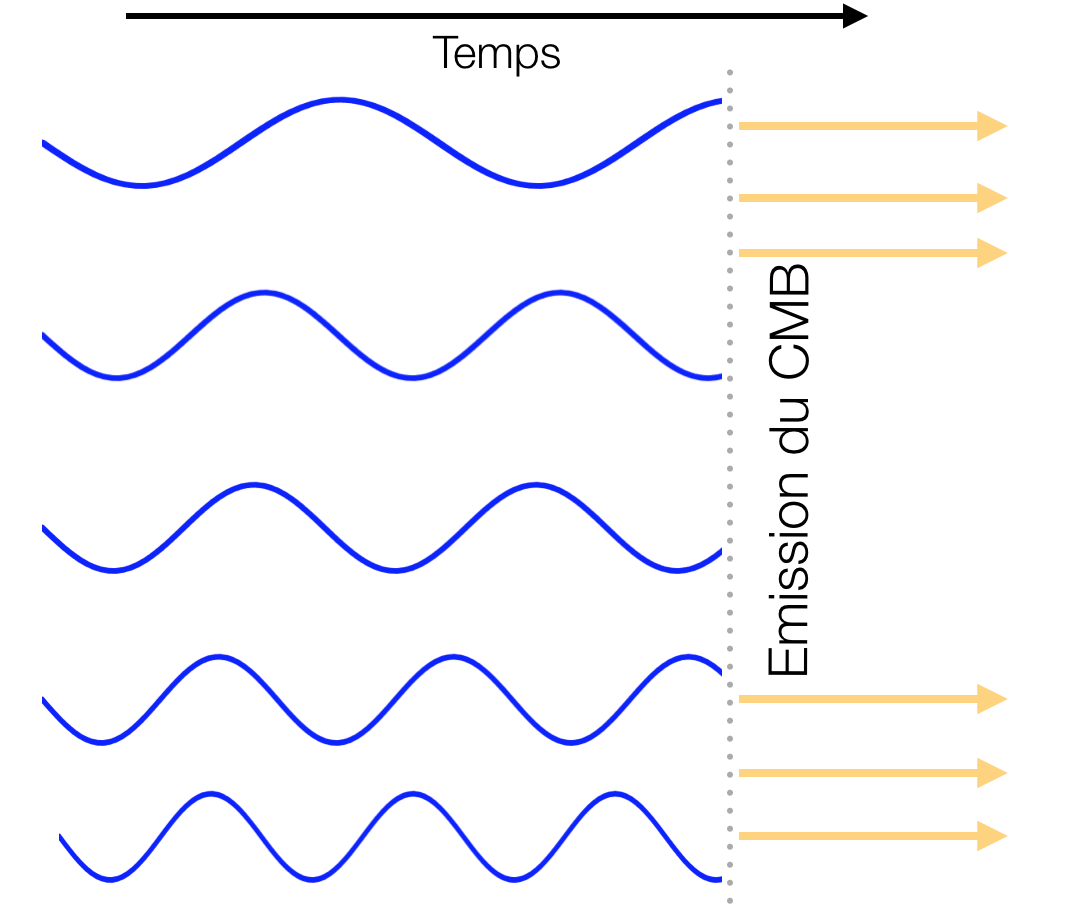
\includegraphics[height=12cm]{figs/bao1.png}
	\caption[Les oscillations baryoniques évoluent sur des fréquences différentes, dépendant de leur taille.]{Les oscillations baryoniques évoluent sur des fréquences différentes, dépendant de leur taille. Les grandes structures oscillent lentement, les petites rapidement. Certains modes vont être en extremum d'amplitude au moment de la Recombinaison et donc au moment de la dernière diffusion du fond diffus cosmologique. Ces modes vont donc être privilégiés dans la carte du CMB.}
	\label{f:bao1}
\end{figure}


\newthought{Ces oscillations baryoniques}  sont des ondes acoustiques\index{onde acoustique baryonique} (BAOs, de l'anglais \textit{baryonic acoustic oscillations})\index{BAO} car elles sont entretenues par l'entrejeu entre gravité et pression (de rayonnement dans le cas présent). Par simple inspection de l'équation différentielle maîtresse, on peut constater que la fréquence d'oscillation dépend de la taille du mode étudié \sidenote{avec $\omega\sim2\pi c_s/\lambda$}: un mode à grande fréquence spatiale implique une fréquence temporelle élevée et vice-versa. Par conséquent, l'amplitude du mode au moment de la Recombinaison va dépendre du mode en question : au moment de l'émission du fond diffus\index{fond diffus cosmologique}, certains modes seront en amplitude maximale, d'autres en amplitude plus modérée. En simplifiant (voir Fig. \ref{f:bao1}), on peut imaginer que certains modes vont osciller un nombre de fois exactement entier entre leur déclenchement et la Recombinaison, parvenant ainsi à un extremum d'amplitude tandis que d'autres seront dans une phase quelconque avec des amplitudes moins remarquables. Les échelles qui se détachent sous la forme de 'pics' dans le spectre de puissance\index{spectre de puissance} du fond diffus cosmologique (voir Fig. \ref{f:bao2}) sont la manifestation de ces modes qui parviennent en extremum d'amplitude au moment où le rayonnement fossile est produit.



\begin{figure}[htbp]
	\centering
		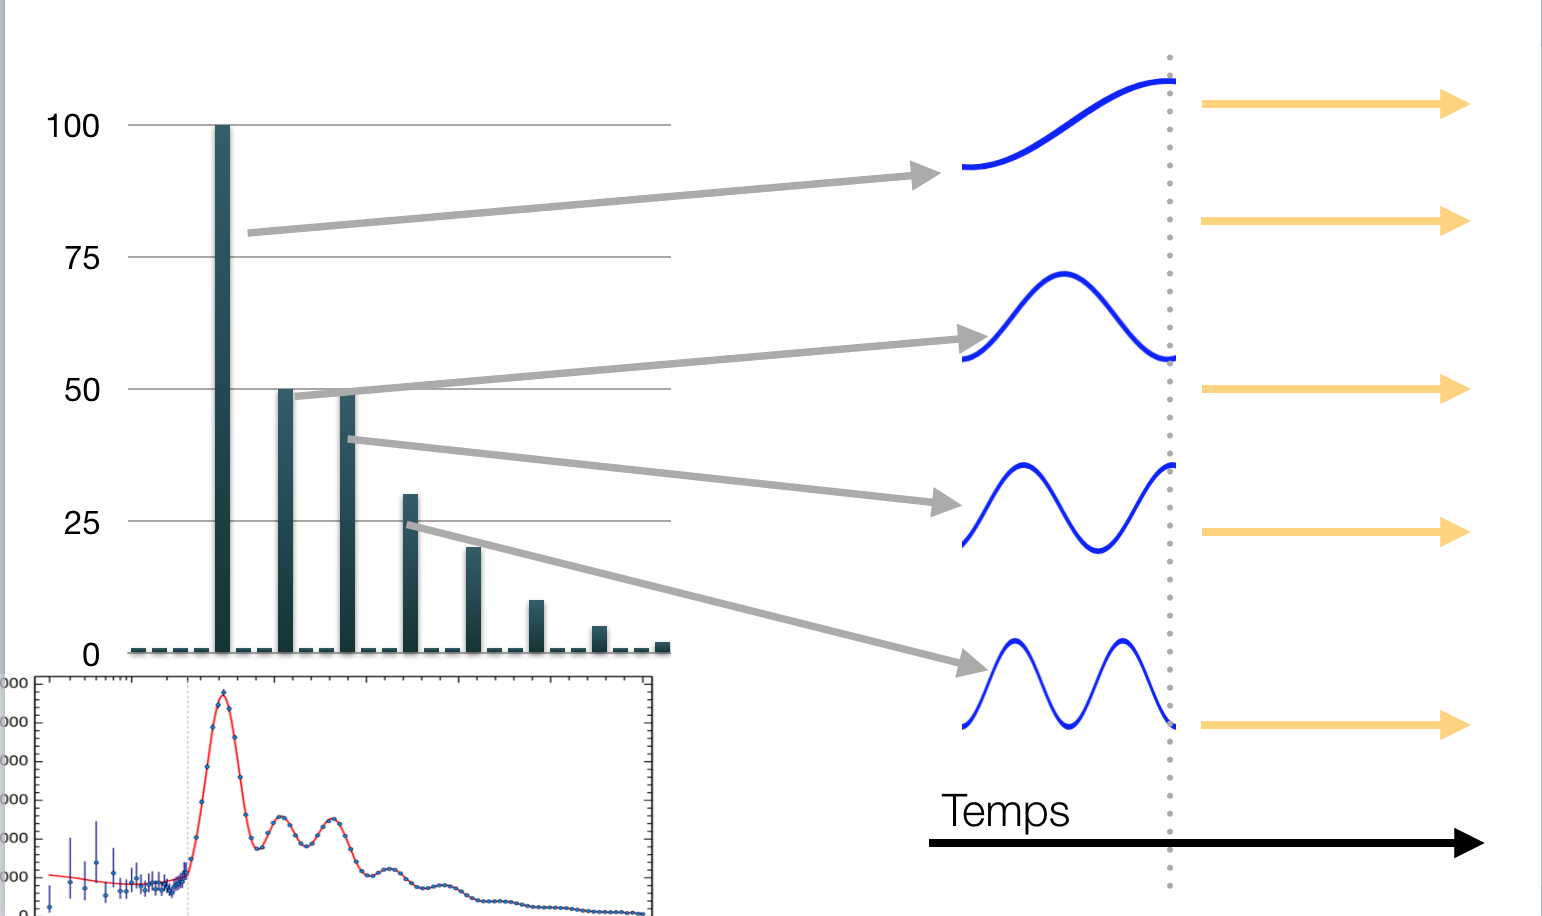
\includegraphics[height=12cm]{figs/bao2.png}
	\caption[Les pics acoustiques sont des extrema]{Les pics acoustiques du spectre de puissance du fond diffus cosmologique correspondent aux modes qui sont en extremum d'amplitude au moment de la Recombinaison. Le premier pic correspond à une compression, le second une compression + une détente, le troisième une compression + une détente + une compression, etc.. Au premier ordre, nous voyons des harmoniques d'un même mode fondamental. }
	\label{f:bao2}
\end{figure}

\section{Croissance des perturbations : cas super-horizon}

Jusqu'à présent, nous nous sommes concentrés sur les petites échelles. Regardons à présente le comportement d'un mode de très grande taille, dont la longueur caractéristique est plus grande que \textit{l'horizon cosmologique}\index{horizon} à l'instant considéré. Ces modes sont appelés super-horizon, tandis que les modes de petite taille précédemment étudiés sont par analogie désignés comme étant sub-horizon.

\newthought{L'horizon}\index{horizon} désigne la plus grande échelle sur laquelle un phénomène de propagation peut opérer. Sa valeur est simplement donnée par :
\begin{equation}
L_H=\frac{c}{H}
\end{equation}
où $H^{-1}$ apparaît comme une mesure de l'âge de l'Univers à un instant donné. L'horizon est donc le produit de la plus grande vitesse par la plus grande durée. Son expression comobile présente une évolution temporelle qui dépend de la période de domination. Durant la période dominée par le rayonnement on a comme horizon comobile\sidenote{avec $H\sim a^{-2}$}:
\begin{equation}
\ell_{H,RD}=\frac{c}{aH}\sim a
\end{equation} 
et durant la période dominée par la matière\sidenote{avec $H\sim a^{-3/2}$}:
\begin{equation}
\ell_{H,MD}\sim\sqrt{a}.
\end{equation}
Dans les 2 cas, l'horizon grandit avec le temps et un mode de taille comobile donnée va donc successivement être plus grand que l'horizon (super-horizon) puis plus petit (sub-horizon) : usuellement, on désigne cette transition par l'expression \textit{passer sous l'horizon}. Le cas super-horizon demande un traitement en relativité générale complet donnant l'équation de croissance des structures suivantes:
\begin{equation}
\ddot \delta_k + 2H \dot \delta_k = \frac{3}{2}H^2(1+w)(1+3w)\delta_k
\end{equation}
où $w=0$ durant l'époque MD et $w=1/3$ durant l'époque RD \sidenote{pour ces échelles plus grandes que l'horizon, la pression ne peut jouer un rôle significatif: baryons et matière noire ont le même comportement}. 

Cette équation est similaire à celle obtenue dans le cas sub-horizon. Pour l'époque de domination de la matière, on retrouve le même taux de croissance que celui obtenu pour la matière noire :
\begin{equation}
\delta_{k,MD}\sim t^{2/3}\sim a(t),
\end{equation}
tandis que durant l'époque de domination du rayonnement on obtient:
\begin{equation}
\delta_{k,RD}\sim t \sim a(t)^2.
\end{equation}
Dans ce cas, le comportement est substantiellement différent de celui obtenu dans le cas sub-horizon: les modes croissent au lieu de stagner. Ceci reflète l'absence d'influence des forces de pression sur ces échelles hors de leur horizon et équivaut à négliger la vitesse du son $c_s$.

\section{Croissance des perturbations : synthèse et spectre de puissance}

La synthèse des résultats précédents pour le cas de la matière noire est présentée dans la figure \ref{f:perturb}. On constate qu'une petite perturbation peut voir son histoire de croissance gelée si elle passe sous l'horizon\index{horizon} durant l'époque dominée par le rayonnement. À l'inverse, un mode de grande longueur d'onde devra attendre la période dominée par la matière pour changer de régime et ne connaîtra pas la phase de non-croissance qu'auront connue les plus petites structures.

\begin{figure}[htbp]
	\centering
		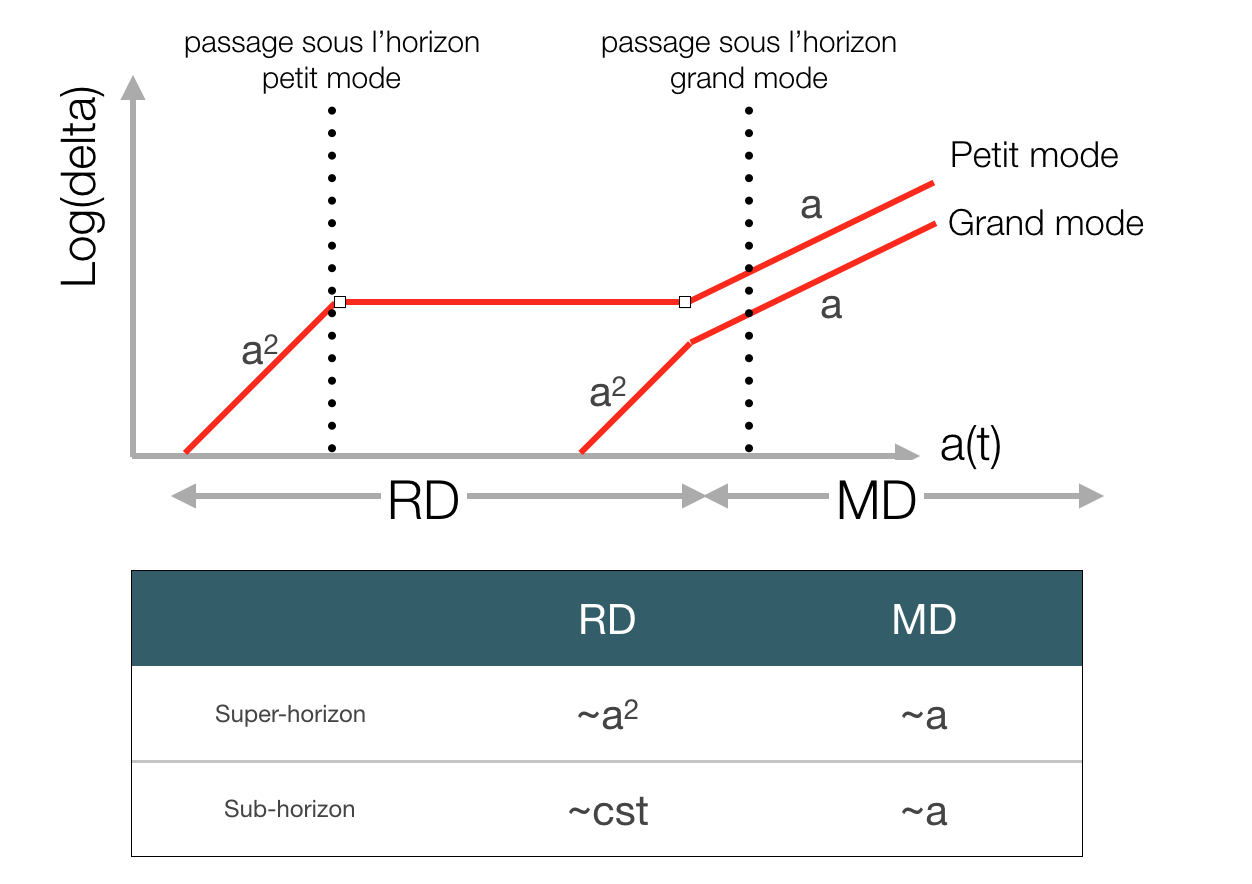
\includegraphics[height=8cm]{figs/perturb.png}
		\caption[Synthèse de la croissance des perturbations]{Synthèse de la croissance des perturbations. Un petit mode possède une taille caractéristique suffisamment petite pour passer sous l'horizon durant l'époque dominée par le rayonnement.}
	\label{f:perturb}
\end{figure}

Grâce à cette synthèse, on peut prédire l'amplitude d'un mode au moment de la Recombinaison $\delta_f$ en fonction de son amplitude $\delta_i$ bien avant l'équivalence matière-rayonnement\index{Equivalence}. Considérons d'abord le cas d'un grand mode, sans période de gel de croissance, son amplitude au moment de l'équivalence est donnée par \sidenote{l'indice $e$ désigne une valeur prise au moment de l'Équivalence}:
\begin{equation}
\delta_e=\frac{a_e^2}{a_i^2}\delta_i.
\end{equation}
Son amplitude finale est alors donnée par :
\begin{equation}
\delta_f=\frac{a_f}{a_e}\delta_e=\frac{a_f a_e}{a_i^2}\delta_i.
\end{equation}
La chose à noter est l'indépendance du facteur reliant l'amplitude initiale et finale vis-à-vis de la taille du mode\sidenote{bien sûr $a_e$ ne dépend pas du mode considéré} : tous les modes vont croître dans les mêmes proportions entre les instants $i$ et $f$. 

Pour les petits modes, la situation est différente. L'amplitude au passage sous l'horizon est donnée par
\begin{equation}
\delta_L=\frac{a_L^2}{a_i^2}\delta_i.
\end{equation}
où $a_L$ est l'instant de passage sous l'horizon. L'amplitude au moment de l'équivalence est identique à $\delta_L$ car la croissance est gelée et l'amplitude finale est alors donnée par:
\begin{equation}
\delta_f=\frac{a_f}{a_e}\delta_e=\frac{a_f}{a_e}\delta_L=\frac{a_L^2 a_f}{a_i^2 a_e}\delta_i.
\end{equation}
Ici le facteur de lien entre $\delta_f$ et $\delta_i$ dépend de $a_L$ et donc de la taille du mode considéré. En effet, cet instant est déterminé par $\lambda = L_{H,RD} \sim a_L$ donc 
\begin{equation}
\delta_f \sim \frac{1}{k^2} \delta_i.
\end{equation}
On a une coupure d'autant plus forte que la fréquence spatiale du mode est élevée, d'autant plus forte que la taille du mode considéré est petite.

\newthought{Pour le spectre de puissance}\index{spectre de Puissance}, les conséquences sont simples. Pour les $k$ suffisamment faibles, donc les grands modes, on a 
\begin{equation}
P_f(k)\sim\delta_k^2 \sim P_i(k),
\end{equation}
par contre pour les hautes fréquences, donc les petits modes, le spectre de puissance est filtré suivant la relation:
\begin{equation}
P_f(k)\sim \frac{1}{k^4} P_i(k)
\end{equation}
Comme le spectre de puissance primordial est en loi de puissance tel que \sidenote{on parle de spectre invariant d'échelle, comme prédit par exemple par les théories d'Inflation\index{Inflation}}:
\begin{equation}
P_i(k)\sim k
\end{equation}
on obtient un spectre caractéristique aux hautes fréquences en 
\begin{equation}
P_f(k)\sim\frac{1}{k^3}.
\end{equation}
Le spectre de puissance résultant possède donc 2 régimes caractéristiques, l'un aux grandes échelles en $P(k)\sim k$ et l'autre aux petites échelles en $P(k)\sim k^{-3}$. La transition entre les deux correspond à l'échelle qui passe sous l'horizon exactement au moment de l'Équivalence\index{Equivalence} (cf. Fig \ref{f:pk}).

\begin{figure}[htbp]
	\centering
		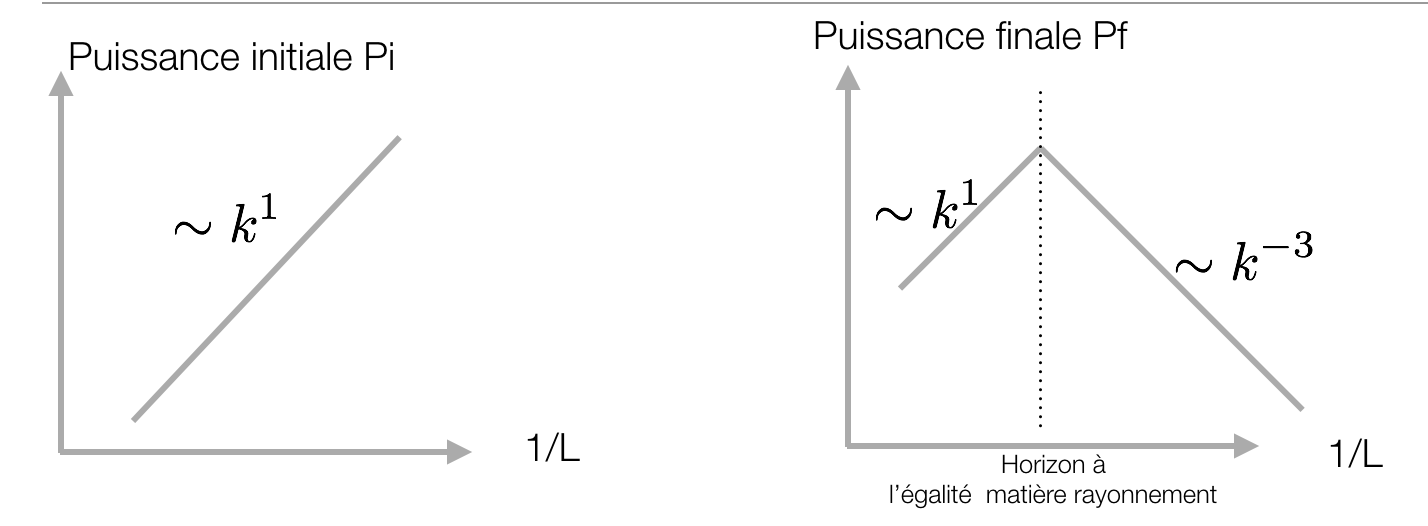
\includegraphics[height=8cm]{figs/pk.png}
		\caption[Schématique du filtrage du spectre de puissance des fluctuations initiales.]{Schématique du filtrage du spectre de puissance des fluctuations initiales. Le spectre primordial est invariant d'échelle en $P(k)\sim k$ et le gel de la croissance des fluctuations sous l'horizon durant l'époque de domination du rayonnement produit un filtrage aux hautes fréquences qui produit une pente caractéristique en $P(k)\sim k^{-3}$.}
	\label{f:pk}
\end{figure}

\newthought{Pour résumer}, le spectre de puissance de la matière est une version filtrée du spectre de puissance primordial. Ce filtre opère sur les échelles suffisamment petites pour passer dans l'Horizon cosmologique tôt dans l'histoire de l'Univers, durant l'époque dominée par le rayonnement. Les échelles plus grandes ne permettant pas ce passage ont crû de façon indifférenciée et ont donc conservé les caractéristiques du spectre primordial. L'ensemble des prédictions développées dans ce chapitre, et notamment la mise en place du spectre de puissance $P(k)$ est fermement confirmée par de multiples observations (voir Fig. \ref{f:pktegmark})~: c'est un des grands succès du modèle $\Lambda$CDM aux grandes échelles.

\begin{figure}[htbp]
	\centering
		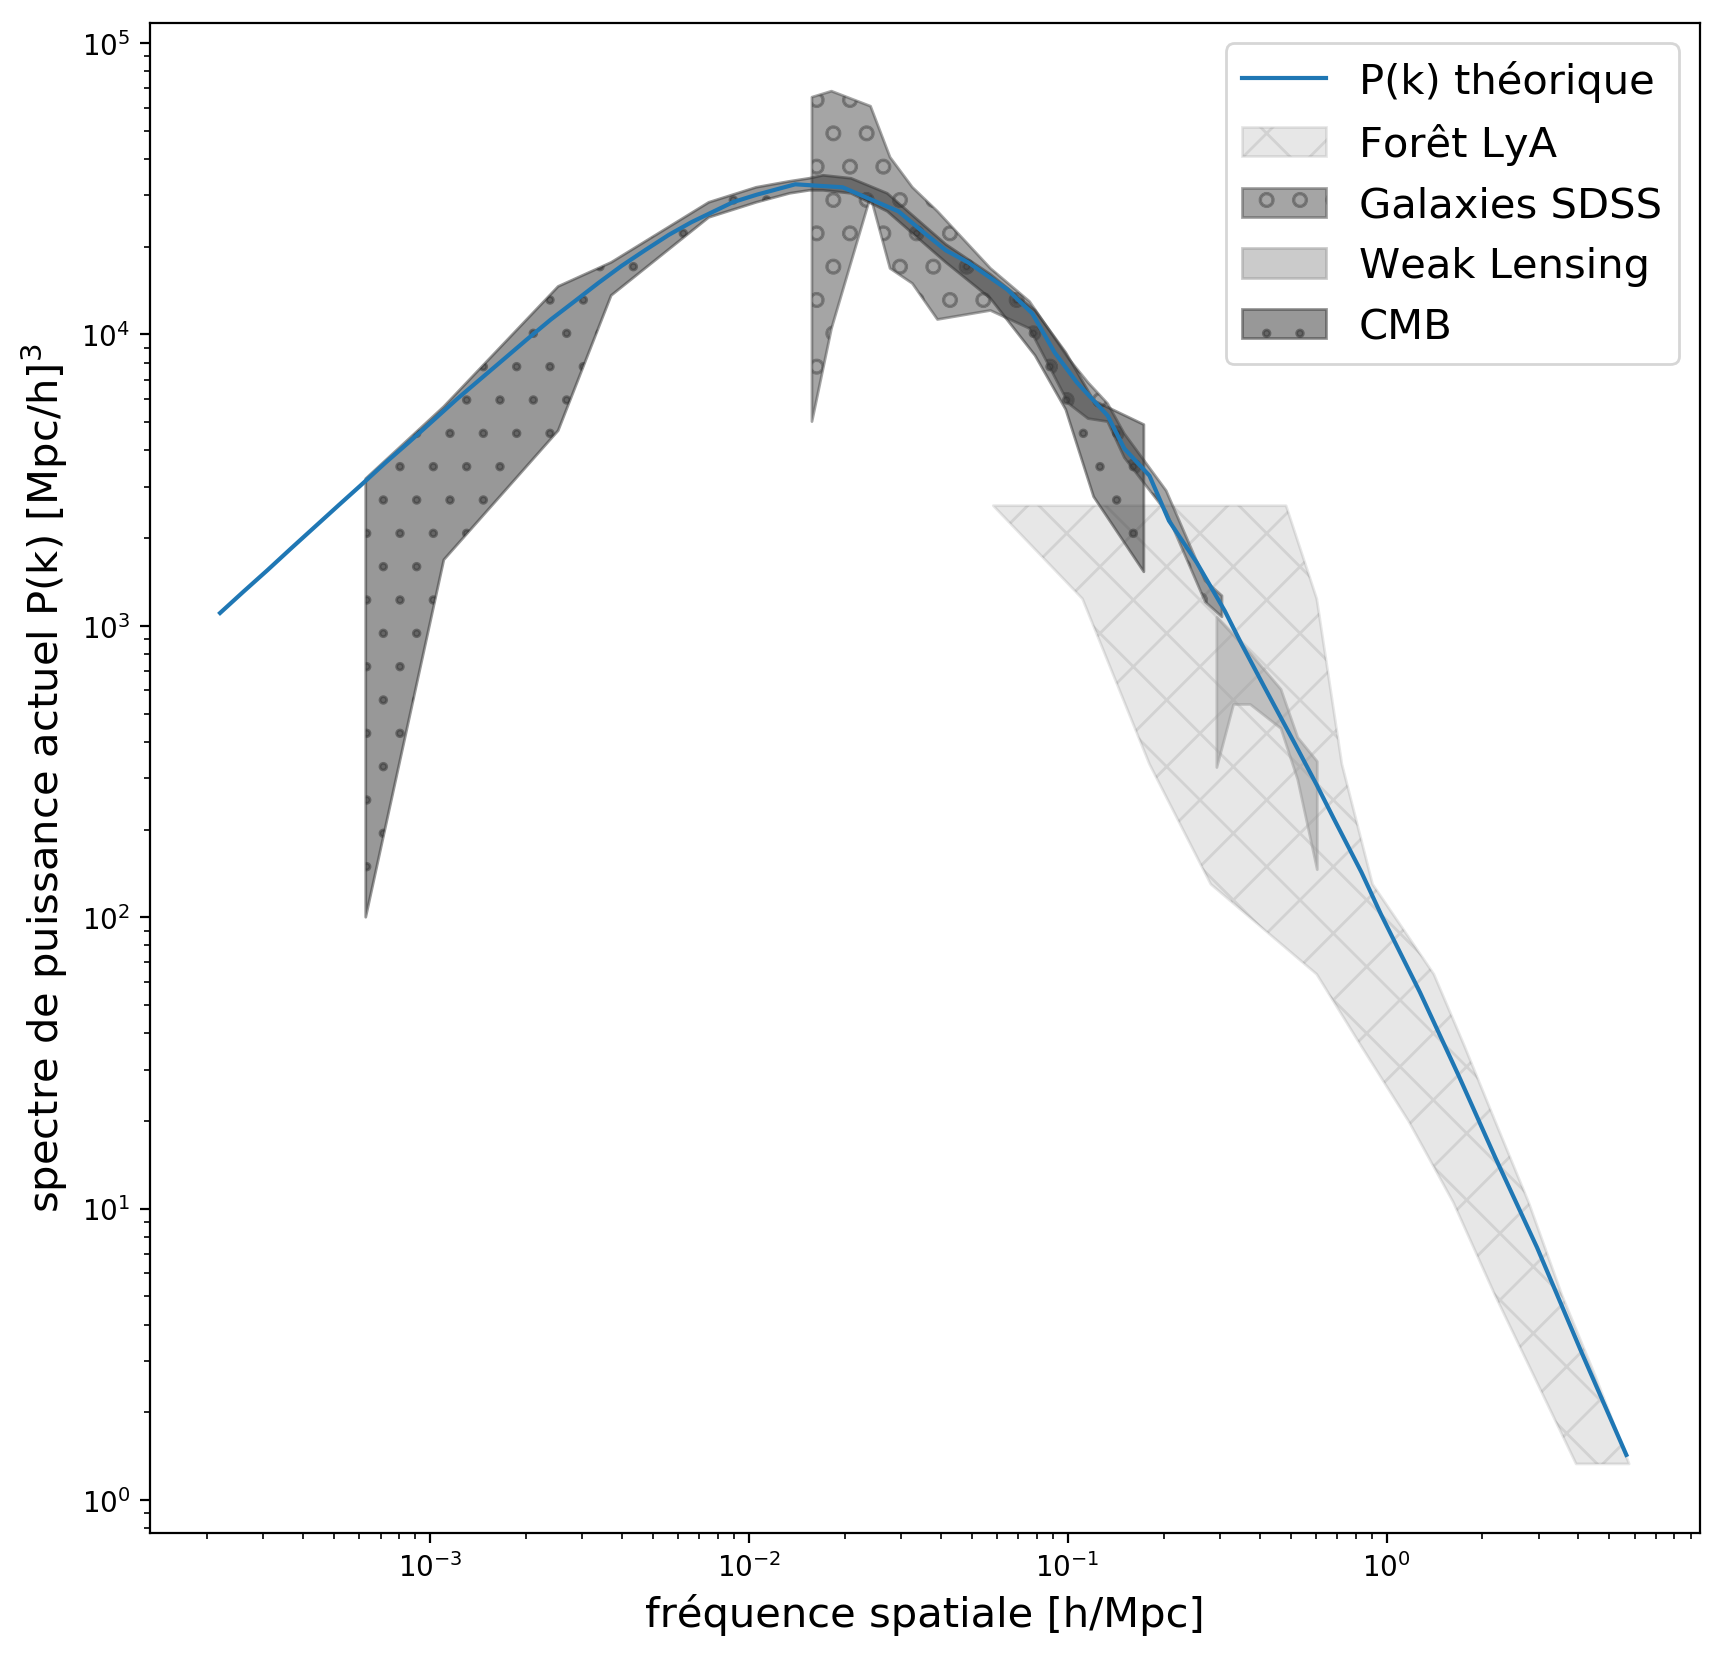
\includegraphics[height=12cm]{figs/pstegmark.png}
		\caption[Le spectre de puissance observé]{Le spectre de puissance $P(k)$ $\Lambda CDM$ théorique est représenté ici avec une compilation des estimations observationnelles issues de différentes sondes~: lensing, relevés de galaxies, CMB, Forêt Lyman-$\alpha$. On note l'excellent accord en théorie et prédiction.  Figure inspirée de Tegmark et al. 2003. }
	\label{f:pktegmark}
\end{figure}


\newthought{Les oscillations baryoniques}\index{BAO}, mentionnées dans le cas de la matière avec pression et vues dans le CMB, se manifestent également dans le spectre de puissance de la matière totale. Ces ondes sonores se propageant dans le gaz vont légèrement modifier la structure globale de la matière : même si les baryons ne représentent qu'une faible fraction\sidenote{$\frac{\Omega_b}{\Omega_m}\sim0.15$} de la masse totale, cette fraction est non nulle et joue sur la dynamique globale à l'œuvre. Ces oscillations se manifestent à nouveau comme des modes légèrement privilégiés dans le spectre de puissance $P(k)$. Par ailleurs, ces modes privilégiés vont persister dans la distribution de matière bien au-delà de la Recombinaison, jusqu'à nos jours. Par exemple, le spectre de puissance de la distribution actuelle des galaxies\sidenote{mesurée à z=0 dans des grands relevés de millions de galaxies comme le Sloan Digital Sky Survey (SDSS)}  présente des modes privilégiés aux fréquences attendues à des niveaux faibles de l'ordre du, $\%$ mais non nuls(voir Fig. \ref{f:percival}). De même, la distribution du gaz diffus intergalactique\index{IGM} à z=2\sidenote{sondée dans les spectres de Quasars distant} manifeste ces mêmes modes privilégiés. Ces ondes de pression primordiales ont laissé leur empreinte dans toutes les structures qui ont émergé tout au long de l'histoire de l'Univers.

\begin{figure}[htbp]
	\centering
		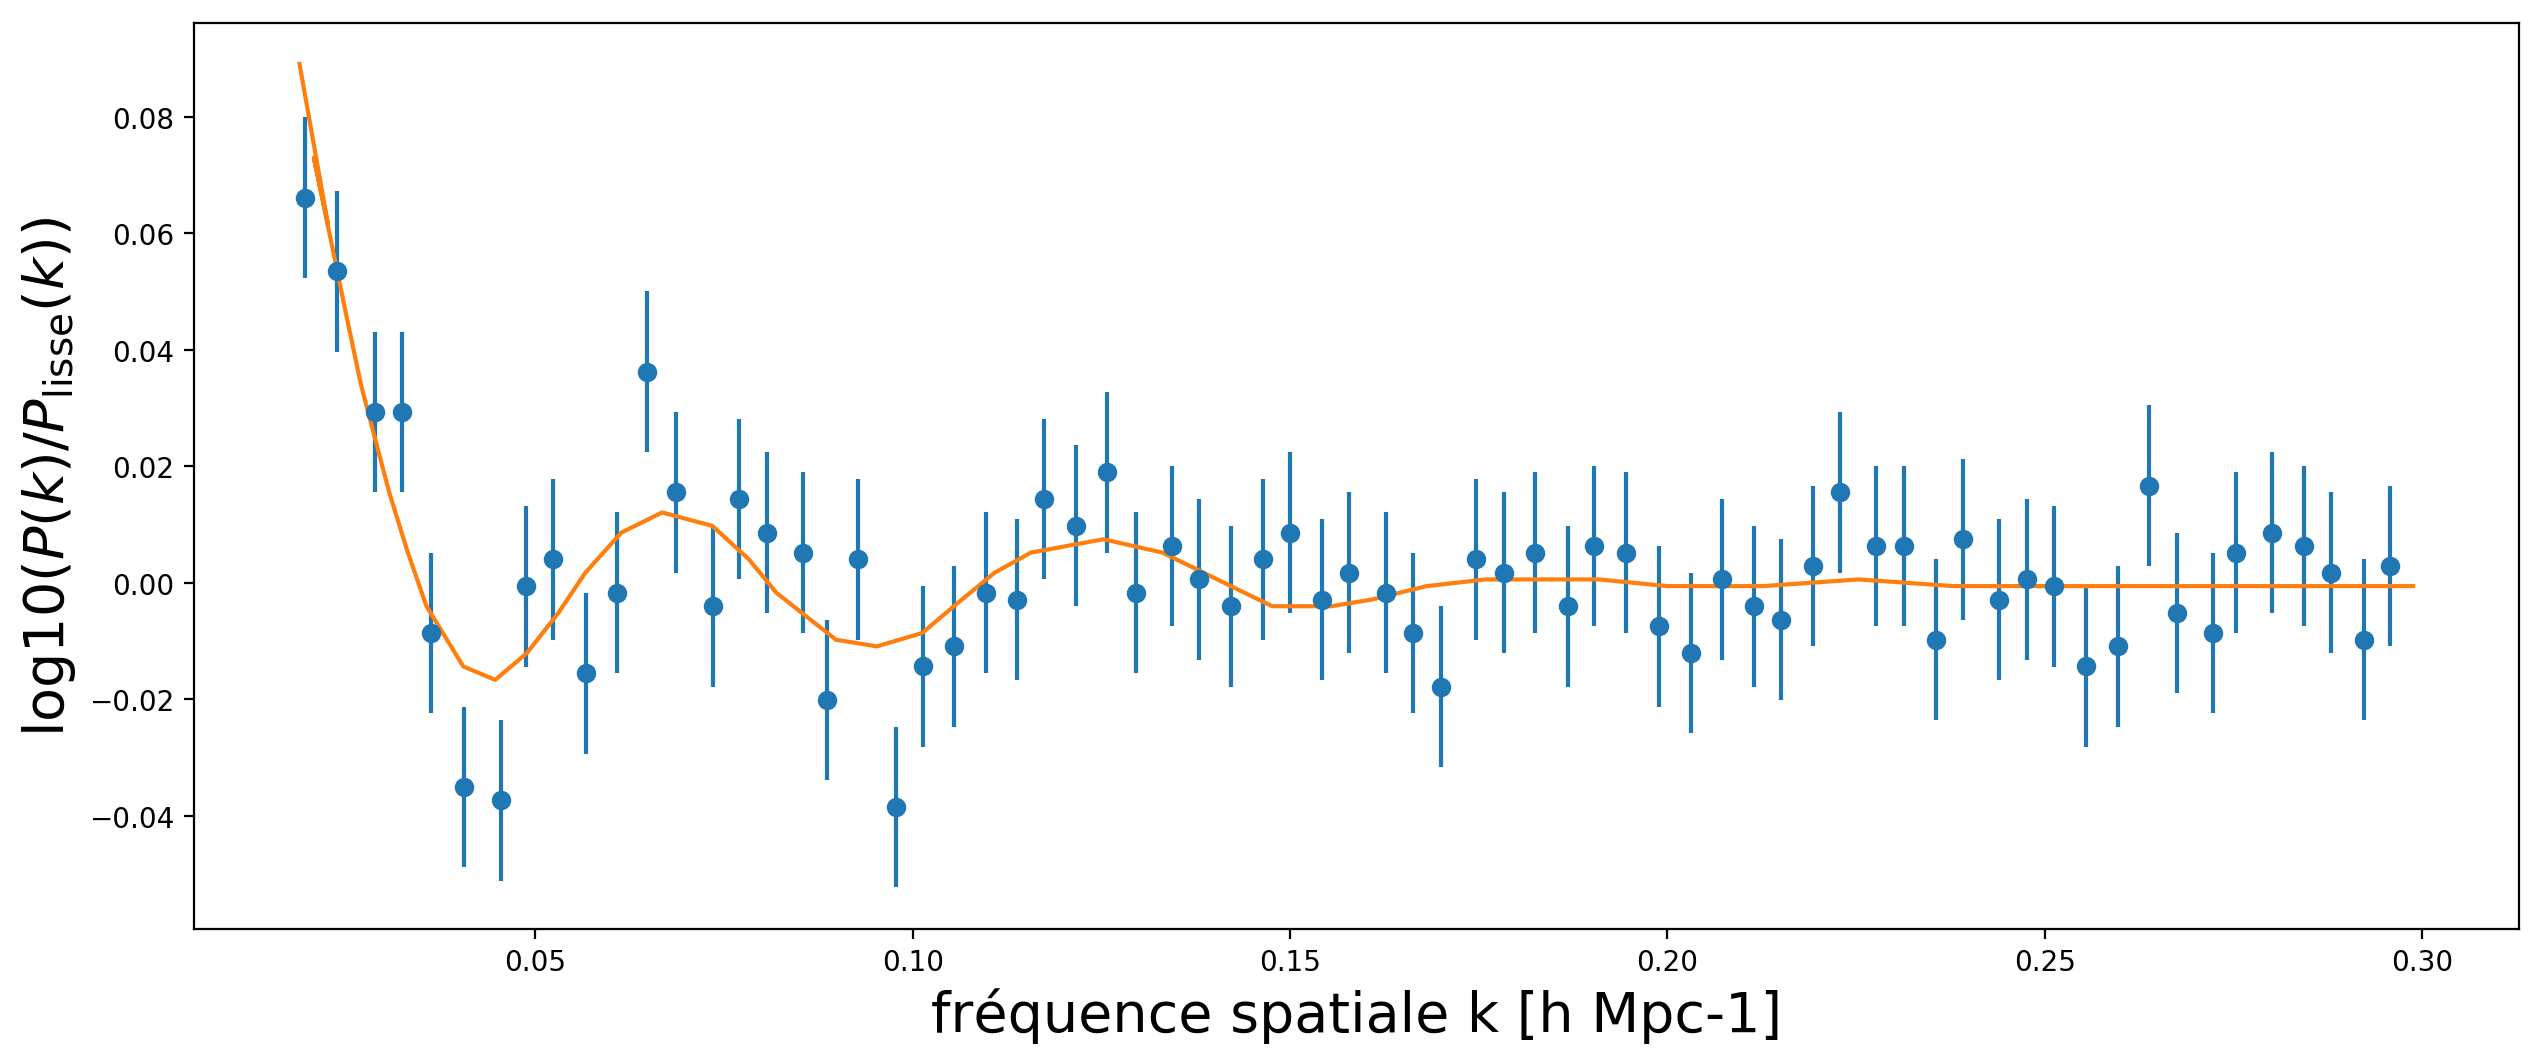
\includegraphics[height=15cm]{figs/percival.png}
		\caption[Les BAOs dans les relevés de galaxies]{Détection des BAOs dans le spectre de puissance du grand relevé de galaxies SDSS. La courbe représentée est le rapport du spectre mesuré dans les données au spectre lissé sans BAOs. Les BAOs sont très clairement apparents (points) aux positions prédites par la théorie (ligne). Figure inspirée de Percival et al. 2007.}
	\label{f:percival}
\end{figure}

\section{Et après ?}

Une fois le mécanisme d'instabilité déclenché, tous les modes vont parvenir à des régimes de surdensité qui vont au-delà du régime linéaire et qui sortent du cadre dans lequel nous nous sommes placés. Dans certains cas académiques, le régime non linéaire\index{régime non-linéaire} peut être abordé analytiquement, mais en toute généralité il requiert l'utilisation de simulations numériques. La culmination de ce régime non linéaire est la création de structures denses, dominées par les baryons et au sein desquelles se forment les sources de rayonnement : ce sont les galaxies qui nous entourent. L'apparition de ces objets est donc conditionnée par un contexte cosmologique et par extension il n'est pas illogique d'affirmer que l'étude de la formation des galaxies\index{formation des galaxies} est une extension naturelle de la cosmologie. Toutefois, des phénomènes astrophysiques commencent à rentrer en jeu aux échelles considérées : thermodynamique du gaz, processus physico-chimique de refroidissement, champ magnétique, formation et rétroaction stellaire, production et impact des éléments plus lourds que l'hélium, etc.. Chacun de ces phénomènes est un objet d'étude à part entière et chacun de ces phénomènes est compris de façon toute relative. On en décrira quelques-uns par la suite, mais de façon générale on peut aisément avancer qu'aujourd'hui l'extension de la théorie cosmologique à celle de la formation des galaxies présente des défis majeurs.À l'heure où ces lignes sont écrites, ces défis ne sont pas résolus.

